\begingroup\fontsize{9}{11}\selectfont

\begin{longtable}[t]{llllrrrrrr}
\caption{\label{tab:arbitrary_trend_table}We run a logistic model regressing success against perturb-target distance and perturb box length, both relative to image width or height, in the deliberate attack experiment. Longer perturb box length or shorter perturb-target distance cause success rates to significantly increase for all model and attack combinations, except for perturb box length in untargeted attack on Cascade R-CNN. The interaction terms, even when significant, are negligibly close to 0. Table headers are explained in Appendix \ref{app:tab_hdr}.}\\
\toprule
\multicolumn{2}{c}{Group} & \multicolumn{8}{c}{Regression} \\
\cmidrule(l{3pt}r{3pt}){1-2} \cmidrule(l{3pt}r{3pt}){3-10}
 & Attack & term & sig & estimate & std.error & statistic & p.value & conf.low & conf.high\\
\midrule
\addlinespace[0.3em]
\multicolumn{10}{l}{\textbf{YOLOv3}}\\
\hspace{1em} & Vanishing & distance & * & -7.152 & 1.243 & -5.753 & 0.000 & -9.610 & -4.734\\
\cmidrule{3-10}\nopagebreak
\hspace{1em} &  & length & * & 7.648 & 0.578 & 13.235 & 0.000 & 6.543 & 8.810\\
\cmidrule{3-10}\nopagebreak
\hspace{1em} &  & distance * length & * & -12.247 & 3.877 & -3.159 & 0.002 & -19.885 & -4.676\\
\cmidrule{2-10}\nopagebreak
\hspace{1em} & Mislabeling & distance & * & -7.541 & 1.239 & -6.087 & 0.000 & -9.993 & -5.135\\
\cmidrule{3-10}\nopagebreak
\hspace{1em} &  & length & * & 6.055 & 0.442 & 13.713 & 0.000 & 5.205 & 6.937\\
\cmidrule{3-10}\nopagebreak
\hspace{1em} &  & distance * length &  & 0.465 & 3.465 & 0.134 & 0.893 & -6.299 & 7.295\\
\cmidrule{2-10}\nopagebreak
\hspace{1em} & Untargeted & distance & * & -9.464 & 1.469 & -6.441 & 0.000 & -12.392 & -6.629\\
\cmidrule{3-10}\nopagebreak
\hspace{1em} &  & length & * & 2.895 & 0.287 & 10.081 & 0.000 & 2.336 & 3.463\\
\cmidrule{3-10}\nopagebreak
\hspace{1em} &  & distance * length &  & 4.370 & 2.862 & 1.527 & 0.127 & -1.201 & 10.021\\
\cmidrule{1-10}\pagebreak[0]
\addlinespace[0.3em]
\multicolumn{10}{l}{\textbf{SSD}}\\
\hspace{1em} & Vanishing & distance & * & -9.986 & 1.267 & -7.881 & 0.000 & -12.501 & -7.532\\
\cmidrule{3-10}\nopagebreak
\hspace{1em} &  & length & * & 4.189 & 0.326 & 12.840 & 0.000 & 3.556 & 4.835\\
\cmidrule{3-10}\nopagebreak
\hspace{1em} &  & distance * length &  & -1.319 & 2.772 & -0.476 & 0.634 & -6.734 & 4.138\\
\cmidrule{2-10}\nopagebreak
\hspace{1em} & Mislabeling & distance & * & -10.593 & 1.354 & -7.826 & 0.000 & -13.284 & -7.975\\
\cmidrule{3-10}\nopagebreak
\hspace{1em} &  & length & * & 5.541 & 0.362 & 15.323 & 0.000 & 4.841 & 6.259\\
\cmidrule{3-10}\nopagebreak
\hspace{1em} &  & distance * length & * & -7.154 & 2.976 & -2.404 & 0.016 & -12.974 & -1.302\\
\cmidrule{2-10}\nopagebreak
\hspace{1em} & Untargeted & distance & * & -10.787 & 1.410 & -7.652 & 0.000 & -13.594 & -8.065\\
\cmidrule{3-10}\nopagebreak
\hspace{1em} &  & length & * & 3.497 & 0.296 & 11.810 & 0.000 & 2.921 & 4.082\\
\cmidrule{3-10}\nopagebreak
\hspace{1em} &  & distance * length &  & 1.528 & 2.835 & 0.539 & 0.590 & -3.998 & 7.119\\
\cmidrule{1-10}\pagebreak[0]
\addlinespace[0.3em]
\multicolumn{10}{l}{\textbf{RetinaNet}}\\
\hspace{1em} & Vanishing & distance & * & -17.682 & 2.722 & -6.496 & 0.000 & -23.208 & -12.539\\
\cmidrule{3-10}\nopagebreak
\hspace{1em} &  & length & * & 3.479 & 0.353 & 9.849 & 0.000 & 2.793 & 4.178\\
\cmidrule{3-10}\nopagebreak
\hspace{1em} &  & distance * length & * & -27.250 & 6.138 & -4.440 & 0.000 & -39.253 & -15.183\\
\cmidrule{2-10}\nopagebreak
\hspace{1em} & Mislabeling & distance & * & -14.139 & 3.516 & -4.022 & 0.000 & -21.420 & -7.626\\
\cmidrule{3-10}\nopagebreak
\hspace{1em} &  & length & * & 2.442 & 0.399 & 6.127 & 0.000 & 1.665 & 3.227\\
\cmidrule{3-10}\nopagebreak
\hspace{1em} &  & distance * length & * & -23.945 & 7.834 & -3.056 & 0.002 & -39.181 & -8.436\\
\cmidrule{2-10}\nopagebreak
\hspace{1em} & Untargeted & distance & * & -15.950 & 2.003 & -7.964 & 0.000 & -19.953 & -12.100\\
\cmidrule{3-10}\nopagebreak
\hspace{1em} &  & length & * & 3.483 & 0.327 & 10.664 & 0.000 & 2.850 & 4.130\\
\cmidrule{3-10}\nopagebreak
\hspace{1em} &  & distance * length & * & 24.373 & 3.645 & 6.687 & 0.000 & 17.330 & 31.623\\
\cmidrule{1-10}\pagebreak[0]
\addlinespace[0.3em]
\multicolumn{10}{l}{\textbf{Faster R-CNN}}\\
\hspace{1em} & Vanishing & distance & * & -19.538 & 3.179 & -6.146 & 0.000 & -26.021 & -13.562\\
\cmidrule{3-10}\nopagebreak
\hspace{1em} &  & length & * & 3.241 & 0.360 & 8.995 & 0.000 & 2.541 & 3.953\\
\cmidrule{3-10}\nopagebreak
\hspace{1em} &  & distance * length & * & -24.042 & 6.889 & -3.490 & 0.000 & -37.462 & -10.448\\
\cmidrule{2-10}\nopagebreak
\hspace{1em} & Mislabeling & distance & * & -18.953 & 3.679 & -5.151 & 0.000 & -26.533 & -12.110\\
\cmidrule{3-10}\nopagebreak
\hspace{1em} &  & length & * & 2.001 & 0.386 & 5.187 & 0.000 & 1.249 & 2.762\\
\cmidrule{3-10}\nopagebreak
\hspace{1em} &  & distance * length &  & -14.029 & 7.793 & -1.800 & 0.072 & -29.166 & 1.402\\
\cmidrule{2-10}\nopagebreak
\hspace{1em} & Untargeted & distance & * & -19.478 & 2.004 & -9.722 & 0.000 & -23.486 & -15.630\\
\cmidrule{3-10}\nopagebreak
\hspace{1em} &  & length & * & 3.007 & 0.310 & 9.694 & 0.000 & 2.404 & 3.620\\
\cmidrule{3-10}\nopagebreak
\hspace{1em} &  & distance * length & * & 26.412 & 3.607 & 7.322 & 0.000 & 19.439 & 33.585\\
\cmidrule{1-10}\pagebreak[0]
\addlinespace[0.3em]
\multicolumn{10}{l}{\textbf{Cascade R-CNN}}\\
\hspace{1em} & Vanishing & distance & * & -24.815 & 3.450 & -7.193 & 0.000 & -31.799 & -18.282\\
\cmidrule{3-10}\nopagebreak
\hspace{1em} &  & length & * & 4.498 & 0.410 & 10.967 & 0.000 & 3.704 & 5.312\\
\cmidrule{3-10}\nopagebreak
\hspace{1em} &  & distance * length & * & -38.766 & 7.932 & -4.887 & 0.000 & -54.349 & -23.234\\
\cmidrule{2-10}\nopagebreak
\hspace{1em} & Mislabeling & distance & * & -28.520 & 4.590 & -6.214 & 0.000 & -37.922 & -19.941\\
\cmidrule{3-10}\nopagebreak
\hspace{1em} &  & length & * & 3.122 & 0.391 & 7.978 & 0.000 & 2.362 & 3.896\\
\cmidrule{3-10}\nopagebreak
\hspace{1em} &  & distance * length & * & -20.448 & 9.401 & -2.175 & 0.030 & -38.672 & -1.816\\
\cmidrule{2-10}\nopagebreak
\hspace{1em} & Untargeted & distance & * & -34.458 & 3.088 & -11.159 & 0.000 & -40.684 & -28.577\\
\cmidrule{3-10}\nopagebreak
\hspace{1em} &  & length & * & 1.746 & 0.314 & 5.556 & 0.000 & 1.134 & 2.367\\
\cmidrule{3-10}\nopagebreak
\hspace{1em} &  & distance * length & * & 39.168 & 5.001 & 7.832 & 0.000 & 29.539 & 49.150\\
\bottomrule
\end{longtable}
\endgroup{}

\begingroup\fontsize{9}{11}\selectfont

\begin{longtable}[t]{llllrrrrrr}
\caption{\label{tab:rand_arb_compare_table}We combined the data in the randomized and deliberate attack experiments to run a logistic model regressing success against object (versus non-object), with perturb-target distance and perturb box size as covariates, both relative to image width or height. The ``object'' term codes object as 1 and non-object as 0. Perturbing an object (in the randomized attack) rather than a non-object (in the deliberate attack) significantly decreases success rates for all model and attack combinations, after controlling for perturb sizes and perturb-target distances. Table headers are explained in Appendix \ref{app:tab_hdr}.}\\
\toprule
\multicolumn{2}{c}{Group} & \multicolumn{8}{c}{Regression} \\
\cmidrule(l{3pt}r{3pt}){1-2} \cmidrule(l{3pt}r{3pt}){3-10}
 & Attack & term & sig & estimate & std.error & statistic & p.value & conf.low & conf.high\\
\midrule
\addlinespace[0.3em]
\multicolumn{10}{l}{\textbf{YOLOv3}}\\
\hspace{1em} & Vanishing & object & * & -0.537 & 0.069 & -7.786 & 0.000 & -0.673 & -0.402\\
\cmidrule{3-10}\nopagebreak
\hspace{1em} &  & distance & * & -9.619 & 0.490 & -19.631 & 0.000 & -10.594 & -8.673\\
\cmidrule{3-10}\nopagebreak
\hspace{1em} &  & size & * & 16.138 & 0.963 & 16.761 & 0.000 & 14.301 & 18.075\\
\cmidrule{3-10}\nopagebreak
\hspace{1em} &  & distance * size & * & -38.994 & 5.279 & -7.387 & 0.000 & -49.534 & -28.837\\
\cmidrule{2-10}\nopagebreak
\hspace{1em} & Mislabeling & object & * & -0.622 & 0.064 & -9.731 & 0.000 & -0.747 & -0.497\\
\cmidrule{3-10}\nopagebreak
\hspace{1em} &  & distance & * & -7.946 & 0.430 & -18.471 & 0.000 & -8.802 & -7.116\\
\cmidrule{3-10}\nopagebreak
\hspace{1em} &  & size & * & 8.275 & 0.521 & 15.875 & 0.000 & 7.275 & 9.319\\
\cmidrule{3-10}\nopagebreak
\hspace{1em} &  & distance * size &  & -5.788 & 3.262 & -1.775 & 0.076 & -12.240 & 0.551\\
\cmidrule{2-10}\nopagebreak
\hspace{1em} & Untargeted & object & * & -0.776 & 0.077 & -10.107 & 0.000 & -0.928 & -0.626\\
\cmidrule{3-10}\nopagebreak
\hspace{1em} &  & distance & * & -10.294 & 0.710 & -14.502 & 0.000 & -11.713 & -8.930\\
\cmidrule{3-10}\nopagebreak
\hspace{1em} &  & size & * & 3.025 & 0.291 & 10.388 & 0.000 & 2.457 & 3.599\\
\cmidrule{3-10}\nopagebreak
\hspace{1em} &  & distance * size & * & 10.204 & 2.615 & 3.902 & 0.000 & 5.096 & 15.352\\
\cmidrule{1-10}\pagebreak[0]
\addlinespace[0.3em]
\multicolumn{10}{l}{\textbf{SSD}}\\
\hspace{1em} & Vanishing & object & * & 0.325 & 0.064 & 5.072 & 0.000 & 0.200 & 0.451\\
\cmidrule{3-10}\nopagebreak
\hspace{1em} &  & distance & * & -12.970 & 0.533 & -24.350 & 0.000 & -14.031 & -11.943\\
\cmidrule{3-10}\nopagebreak
\hspace{1em} &  & size & * & 5.319 & 0.378 & 14.081 & 0.000 & 4.590 & 6.071\\
\cmidrule{3-10}\nopagebreak
\hspace{1em} &  & distance * size &  & 1.653 & 2.648 & 0.624 & 0.533 & -3.560 & 6.824\\
\cmidrule{2-10}\nopagebreak
\hspace{1em} & Mislabeling & object &  & -0.101 & 0.064 & -1.585 & 0.113 & -0.226 & 0.024\\
\cmidrule{3-10}\nopagebreak
\hspace{1em} &  & distance & * & -11.732 & 0.553 & -21.216 & 0.000 & -12.834 & -10.666\\
\cmidrule{3-10}\nopagebreak
\hspace{1em} &  & size & * & 6.651 & 0.403 & 16.492 & 0.000 & 5.873 & 7.454\\
\cmidrule{3-10}\nopagebreak
\hspace{1em} &  & distance * size & * & -9.854 & 2.818 & -3.497 & 0.000 & -15.407 & -4.359\\
\cmidrule{2-10}\nopagebreak
\hspace{1em} & Untargeted & object &  & 0.027 & 0.064 & 0.424 & 0.672 & -0.098 & 0.152\\
\cmidrule{3-10}\nopagebreak
\hspace{1em} &  & distance & * & -12.646 & 0.597 & -21.177 & 0.000 & -13.838 & -11.497\\
\cmidrule{3-10}\nopagebreak
\hspace{1em} &  & size & * & 3.258 & 0.291 & 11.201 & 0.000 & 2.693 & 3.834\\
\cmidrule{3-10}\nopagebreak
\hspace{1em} &  & distance * size & * & 7.145 & 2.448 & 2.919 & 0.004 & 2.344 & 11.942\\
\cmidrule{1-10}\pagebreak[0]
\addlinespace[0.3em]
\multicolumn{10}{l}{\textbf{RetinaNet}}\\
\hspace{1em} & Vanishing & object & * & -0.251 & 0.085 & -2.953 & 0.003 & -0.418 & -0.085\\
\cmidrule{3-10}\nopagebreak
\hspace{1em} &  & distance & * & -28.371 & 1.624 & -17.466 & 0.000 & -31.631 & -25.264\\
\cmidrule{3-10}\nopagebreak
\hspace{1em} &  & size & * & 3.453 & 0.360 & 9.591 & 0.000 & 2.755 & 4.167\\
\cmidrule{3-10}\nopagebreak
\hspace{1em} &  & distance * size &  & -5.791 & 5.990 & -0.967 & 0.334 & -17.676 & 5.813\\
\cmidrule{2-10}\nopagebreak
\hspace{1em} & Mislabeling & object &  & -0.164 & 0.113 & -1.447 & 0.148 & -0.388 & 0.057\\
\cmidrule{3-10}\nopagebreak
\hspace{1em} &  & distance & * & -28.622 & 2.391 & -11.973 & 0.000 & -33.480 & -24.110\\
\cmidrule{3-10}\nopagebreak
\hspace{1em} &  & size & * & 2.030 & 0.412 & 4.926 & 0.000 & 1.224 & 2.840\\
\cmidrule{3-10}\nopagebreak
\hspace{1em} &  & distance * size &  & -6.022 & 8.891 & -0.677 & 0.498 & -23.711 & 11.158\\
\cmidrule{2-10}\nopagebreak
\hspace{1em} & Untargeted & object & * & -0.403 & 0.079 & -5.130 & 0.000 & -0.558 & -0.250\\
\cmidrule{3-10}\nopagebreak
\hspace{1em} &  & distance & * & -11.268 & 0.818 & -13.768 & 0.000 & -12.910 & -9.702\\
\cmidrule{3-10}\nopagebreak
\hspace{1em} &  & size & * & 3.662 & 0.292 & 12.542 & 0.000 & 3.092 & 4.237\\
\cmidrule{3-10}\nopagebreak
\hspace{1em} &  & distance * size & * & 26.886 & 2.757 & 9.753 & 0.000 & 21.555 & 32.364\\
\cmidrule{1-10}\pagebreak[0]
\addlinespace[0.3em]
\multicolumn{10}{l}{\textbf{Faster R-CNN}}\\
\hspace{1em} & Vanishing & object & * & -0.618 & 0.104 & -5.964 & 0.000 & -0.823 & -0.416\\
\cmidrule{3-10}\nopagebreak
\hspace{1em} &  & distance & * & -27.236 & 1.889 & -14.422 & 0.000 & -31.047 & -23.643\\
\cmidrule{3-10}\nopagebreak
\hspace{1em} &  & size & * & 3.369 & 0.388 & 8.671 & 0.000 & 2.614 & 4.137\\
\cmidrule{3-10}\nopagebreak
\hspace{1em} &  & distance * size & * & -19.812 & 7.379 & -2.685 & 0.007 & -34.469 & -5.530\\
\cmidrule{2-10}\nopagebreak
\hspace{1em} & Mislabeling & object & * & -0.758 & 0.131 & -5.767 & 0.000 & -1.019 & -0.504\\
\cmidrule{3-10}\nopagebreak
\hspace{1em} &  & distance & * & -22.755 & 2.115 & -10.757 & 0.000 & -27.063 & -18.771\\
\cmidrule{3-10}\nopagebreak
\hspace{1em} &  & size & * & 2.001 & 0.412 & 4.857 & 0.000 & 1.194 & 2.810\\
\cmidrule{3-10}\nopagebreak
\hspace{1em} &  & distance * size &  & -14.270 & 8.311 & -1.717 & 0.086 & -30.831 & 1.768\\
\cmidrule{2-10}\nopagebreak
\hspace{1em} & Untargeted & object & * & -0.296 & 0.080 & -3.719 & 0.000 & -0.452 & -0.140\\
\cmidrule{3-10}\nopagebreak
\hspace{1em} &  & distance & * & -11.447 & 0.779 & -14.701 & 0.000 & -13.004 & -9.953\\
\cmidrule{3-10}\nopagebreak
\hspace{1em} &  & size & * & 3.748 & 0.304 & 12.322 & 0.000 & 3.155 & 4.347\\
\cmidrule{3-10}\nopagebreak
\hspace{1em} &  & distance * size & * & 27.445 & 2.829 & 9.703 & 0.000 & 21.965 & 33.056\\
\cmidrule{1-10}\pagebreak[0]
\addlinespace[0.3em]
\multicolumn{10}{l}{\textbf{Cascade R-CNN}}\\
\hspace{1em} & Vanishing & object & * & -0.779 & 0.097 & -7.999 & 0.000 & -0.971 & -0.589\\
\cmidrule{3-10}\nopagebreak
\hspace{1em} &  & distance & * & -29.119 & 1.854 & -15.710 & 0.000 & -32.850 & -25.584\\
\cmidrule{3-10}\nopagebreak
\hspace{1em} &  & size & * & 5.752 & 0.446 & 12.907 & 0.000 & 4.894 & 6.642\\
\cmidrule{3-10}\nopagebreak
\hspace{1em} &  & distance * size & * & -55.876 & 8.604 & -6.494 & 0.000 & -73.094 & -39.336\\
\cmidrule{2-10}\nopagebreak
\hspace{1em} & Mislabeling & object & * & -0.616 & 0.110 & -5.592 & 0.000 & -0.833 & -0.401\\
\cmidrule{3-10}\nopagebreak
\hspace{1em} &  & distance & * & -31.146 & 2.387 & -13.046 & 0.000 & -35.990 & -26.630\\
\cmidrule{3-10}\nopagebreak
\hspace{1em} &  & size & * & 3.180 & 0.381 & 8.347 & 0.000 & 2.438 & 3.933\\
\cmidrule{3-10}\nopagebreak
\hspace{1em} &  & distance * size & * & -24.457 & 9.159 & -2.670 & 0.008 & -42.647 & -6.724\\
\cmidrule{2-10}\nopagebreak
\hspace{1em} & Untargeted & object & * & -0.328 & 0.089 & -3.701 & 0.000 & -0.502 & -0.155\\
\cmidrule{3-10}\nopagebreak
\hspace{1em} &  & distance & * & -17.329 & 1.148 & -15.089 & 0.000 & -19.637 & -15.134\\
\cmidrule{3-10}\nopagebreak
\hspace{1em} &  & size & * & 2.749 & 0.298 & 9.221 & 0.000 & 2.166 & 3.335\\
\cmidrule{3-10}\nopagebreak
\hspace{1em} &  & distance * size & * & 22.929 & 3.289 & 6.972 & 0.000 & 16.523 & 29.419\\
\bottomrule
\end{longtable}
\endgroup{}

\begin{figure}[tb]

{\centering 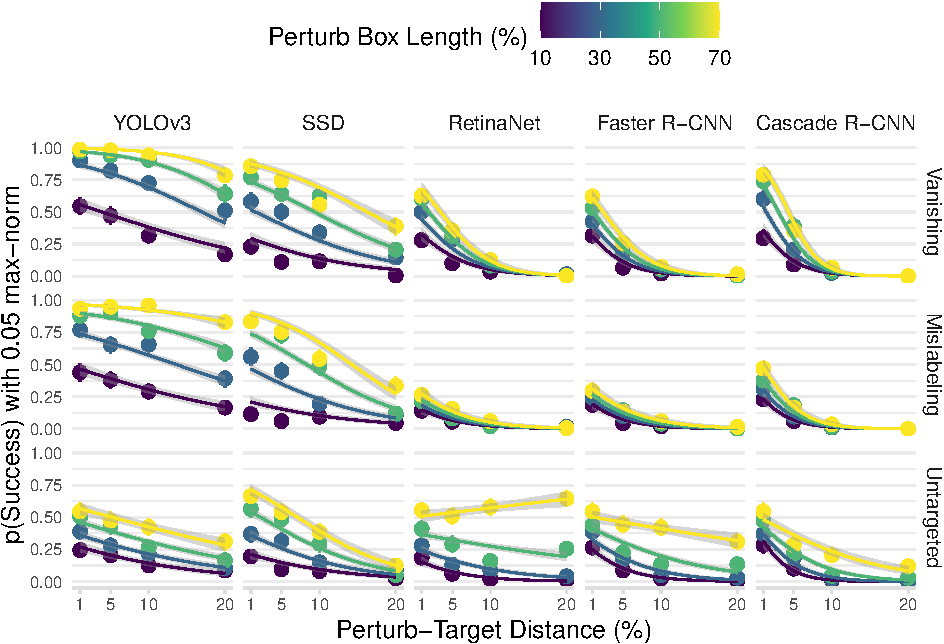
\includegraphics[width=1\linewidth]{imgs-normed/arbitrary_trend_graph-normed} 

}

\caption{Perturbing an arbitrary region obfuscates intent with increased success for all models and attacks even with 0.05 max-norm:  We implement intent obfuscating attack by perturbing an arbitrary non-overlapping square region to disrupt a randomly selected target object at various lengths and distances. The binned summaries and regression trendlines graph success proportion against perturb-target distance and perturb box length, both relative to image width or height, in the deliberate attack experiment. Errors are 95\% confidence intervals and every point aggregates success over 200 images. The deliberate attack multiplies success as compared to the randomized attack (Figure \ref{fig:success_trend_graph}), especially at close perturb-target distance and large perturb box length. Full details are given in Section \ref{sec:del_arb}.}\label{fig:arbitrary_trend_graph_normed}
\end{figure}

\end{document}
